%%%%%%%%%%%%%%%%%%%%%%%%%%%%%%%%%%%%%%%%%
% Journal Article
% LaTeX Template
% Version 1.3 (9/9/13)
%
% This template has been downloaded from:
% http://www.LaTeXTemplates.com
%
% Original author:
% Frits Wenneker (http://www.howtotex.com)
%
% License:
% CC BY-NC-SA 3.0 (http://creativecommons.org/licenses/by-nc-sa/3.0/)
%
%%%%%%%%%%%%%%%%%%%%%%%%%%%%%%%%%%%%%%%%%

%----------------------------------------------------------------------------------------
%	PACKAGES AND OTHER DOCUMENT CONFIGURATIONS
%----------------------------------------------------------------------------------------

\documentclass[twoside]{article}
\usepackage[hyphens]{url} 
\def\UrlBreaks{\do/\do-} % For URL
\usepackage{indentfirst}
\usepackage{lipsum} % Package to generate dummy text throughout this template
\usepackage{graphicx}
\usepackage[sc]{mathpazo} % Use the Palatino font
\usepackage[T1]{fontenc} % Use 8-bit encoding that has 256 glyphs
\linespread{1.05} % Line spacing - Palatino needs more space between lines
\usepackage{microtype} % Slightly tweak font spacing for aesthetics

\usepackage[hmarginratio=1:1,top=32mm,columnsep=20pt]{geometry} % Document margins
\usepackage{multicol} % Used for the two-column layout of the document
\usepackage[hang, small,labelfont=bf,up,textfont=it,up]{caption} % Custom captions under/above floats in tables or figures
\usepackage{booktabs} % Horizontal rules in tables
\usepackage{float} % Required for tables and figures in the multi-column environment - they need to be placed in specific locations with the [H] (e.g. \begin{table}[H])
\usepackage{hyperref} % For hyperlinks in the PDF

\providecommand{\keywords}[1]
{
  \small
  \textbf{\textit{Mots clés---}} #1
}

\usepackage{lettrine} % The lettrine is the first enlarged letter at the beginning of the text
\usepackage{paralist} % Used for the compactitem environment which makes bullet points with less space between them

\usepackage{abstract} % Allows abstract customization
\renewcommand{\abstractnamefont}{\normalfont\bfseries} % Set the "Abstract" text to bold
\renewcommand{\abstracttextfont}{\normalfont\small\itshape} % Set the abstract itself to small italic text

\usepackage{titlesec} % Allows customization of titles
\renewcommand\thesection{\Roman{section}} % Roman numerals for the sections
\renewcommand\thesubsection{\Roman{subsection}} % Roman numerals for subsections
\titleformat{\section}[block]{\large\scshape\centering}{\thesection.}{1em}{} % Change the look of the section titles
\titleformat{\subsection}[block]{\large}{\thesubsection.}{1em}{} % Change the look of the section titles

\usepackage{fancyhdr} % Headers and footers
\pagestyle{fancy} % All pages have headers and footers
\fancyhead{} % Blank out the default header
\fancyfoot{} % Blank out the default footer
\fancyhead[C]{Locker Cracker $\bullet$ June 2020} % Custom header text
\fancyfoot[RO,LE]{\thepage} % Custom footer text

%----------------------------------------------------------------------------------------
%	TITLE SECTION
%----------------------------------------------------------------------------------------

\title{\vspace{-15mm}\fontsize{24pt}{10pt}\selectfont\textbf{Locker Cracker}} % Article title

\author{
\large
\textsc{Denbroeder Audric}\\[2mm] % Your name
\normalsize HE2B - ISIB \\ % Your institution
\normalsize \href{mailto:audric96@gmail.com}{audric96@gmail.com} % Your email address
\vspace{-5mm}
}
\date{}

%----------------------------------------------------------------------------------------

\begin{document}

\maketitle % Insert title

\thispagestyle{fancy} % All pages have headers and footers

%----------------------------------------------------------------------------------------
%	ABSTRACT
%----------------------------------------------------------------------------------------

\begin{abstract}

\keywords{Cadenas, servomoteur, modèle 3D, OCR, tesseract, raspberry pi}

\end{abstract}

%----------------------------------------------------------------------------------------
%	ARTICLE CONTENTS
%----------------------------------------------------------------------------------------

\begin{multicols}{2} % Two-column layout throughout the main article text

\section{Introduction}
Pour le cours de projet et bureau d'étude il m'a été demandé de réaliser un "hacker" de code de cadenas manuel. Ce genre de "robot" existant déjà pour un cadenas de type circulaire, je devais le réaliser sur un cadenas style européen, c'est-à-dire un simple cadenas avec 3-4 chiffres allant de 0 à 9. La façon de réaliser ce projet était libre, je n'avais aucune contrainte, si ce n'est d'utiliser un moteur.
Je vais donc expliquer ici les différentes parties de projet qui sont les suivantes :
\begin{compactitem}
\item L'électronique
\item La modélisation 3D
\item L'informatique
\end{compactitem}

%------------------------------------------------

\section{Electronique}
Dès le début du projet un choix à du être posé : Comment faire pour tourner les chiffres du cadenas. Deux solutions ont été retenues. La première était d'utiliser un moteur utilisant des pinces pour tenir les chiffres et ensuite de faire tourner soit le cadenas soit les pinces pour que les chiffres tournent. Un peu comme un humain le ferait avec 2 doigts. La deuxième était d'utiliser un moteur avec une roue, que l'on mettrait juste à côté des chiffres, en faisant tourner la roue, la roue des chiffres tourneraient avec.

J'ai donc testé les deux solutions très rapidement après le début du projet. Finalement la deuxième solution était bien plus prometteuse que la première, les pinces n'avaient pas assez de couple disponible pour pouvoir tenir la roue du cadenas et la faire tourner en même temps. Cependant la roue n'avait aucun problème pour faire tourner les chiffres.
Le moteur utilisé est le : FS5103R. La roue ayant été utilisée durant ce test est celle disponible avec le servomoteur.

Après avoir réalisé le modèle 3D (cela sera expliqué par la suite), un problème est survenu : L'adhésion de la roue à la roue du chiffre du cadenas. Celle-ci n'était pas parfaite ce qui avait pour conséquence de ne pas faire tourner les chiffres de manière constante. En effet cela se faisait parfois de la bonne façon on passait de 0 à 1 puis à 2, mais à d'autre moment l'adhésion n'étant plus parfaite, le chiffre passait de 2 à 4 ou simplement de 2 à 2.5 (La position milieu bloquant le cadenas).

Pour pallier ce problème mes professeurs m'ont suggéré l'idée d'utiliser une reconnaissance d'image pour lire les chiffres du cadenas. L'idée est que cela ne soit plus le servomoteur qui soit le cerveau et dicte la "cadence", à savoir faire du chiffre par chiffre. Mais plutôt la reconnaissance d'image, celle-ci regardera si il y'a un chiffre : Si non on demande au servomoteur d'avancer, si oui on vérifie le code.

Le projet qui se passait pour le moment sur Arduino utilisera donc une Raspberry Pi afin d'utiliser la camera de celle-ci pour la reconnaissance d'image (Qui sera expliqué plus en détail dans la partie informatique)

Pour faciliter la reconnaissance d'image un "flash" sera présent sur le modèle 3D, ce flash est constitué de LED. Les différentes parties de l'électronique est donc constitué de : 

\begin{compactitem}
\item Une raspberry pi
\item Des leds
\item Un servo-moteur (par rangée de chiffre)
\end{compactitem}

%------------------------------------------------

\section{Modélisation 3D}
La modélisation 3D était une grande partie de ce projet car elle prenait beaucoup de temps durant le développement. En premier lui j'ai dû modéliser un caisson pour tenir le cadenas et le servomoteur proche l'un de l'autre, de façon à ce que la roue du servo soit collée à la roue des chiffres. Pour cela j'ai du aussi modéliser le cadenas : 
\begin{figure}[H]
\centering
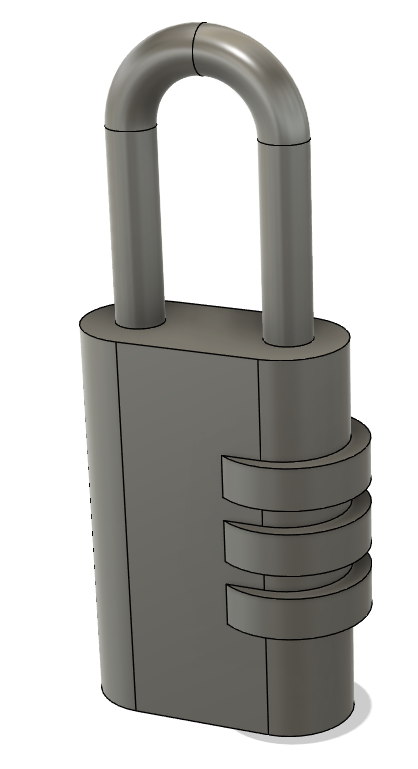
\includegraphics[scale=0.3]{locker.png}
\caption{Modèle 3D du cadenas}
\end{figure}
Ainsi que de modéliser le servomoteur et sa roue : 

\begin{figure}[H]
\centering
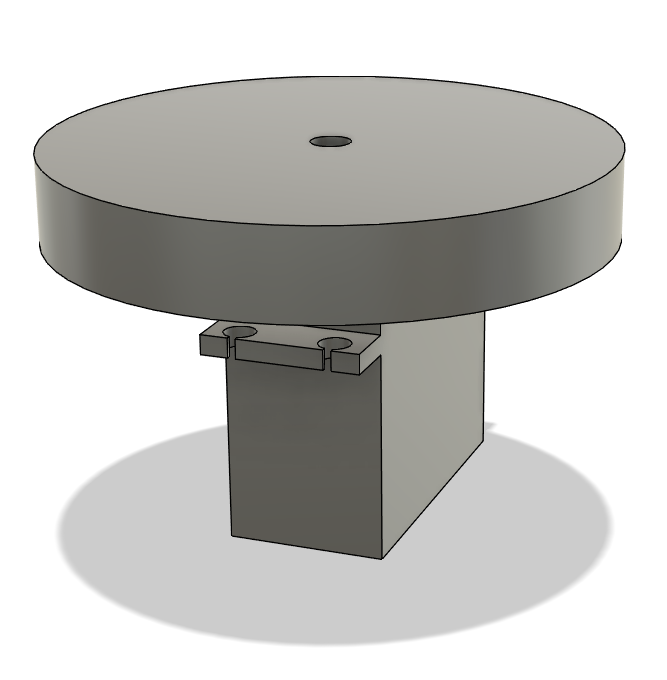
\includegraphics[scale=0.3]{FS5103R_BasicWheels.png}
\caption{Modèle FS5103R}
\end{figure}
Pour avoir au final le 1er modèle : 

\begin{figure}[H]
\centering
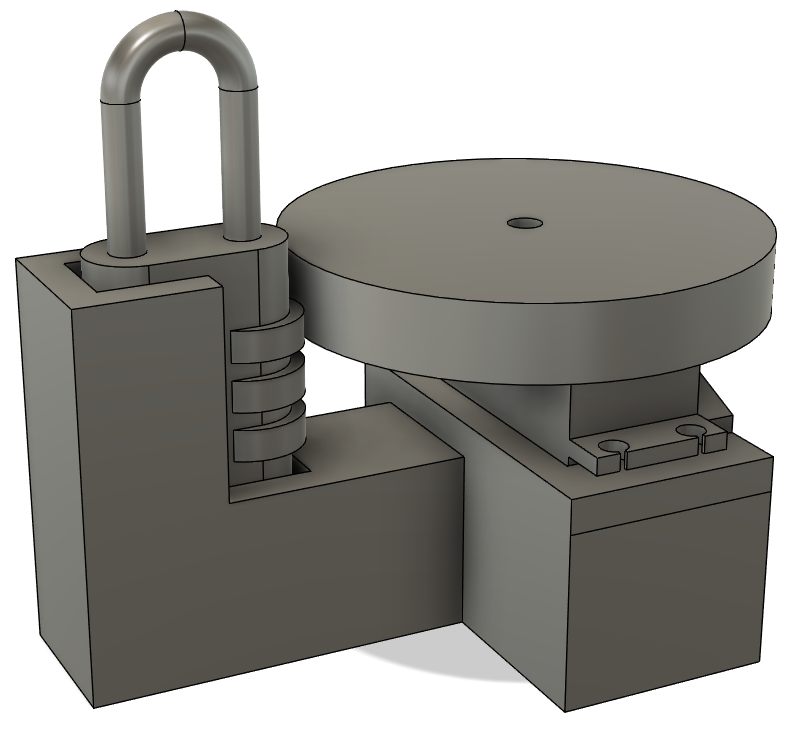
\includegraphics[scale=0.3]{1stStructure.png}
\caption{Modèle FS5103R}
\end{figure}

C'est avec ce modèle que le problème d'adhésion a été détecté, en effet sans ce modèle il est impossible de savoir si l'adhésion est problématique. La cause est que l'on pourrait mal tenir le servomoteur et le cadenas l'un à côté de l'autre.

La réalisation de ce modèle a aussi permis de découvrir que la roue par défaut était beaucoup trop large, en effet celle-ci empiète sur l'une des deux autres rangée de chiffre lorsque mise sur celle du milieu. La solution a donc été de modéliser des nouvelles roues en 3D.

Malheureusement l'engrenage du servomoteur sur lequel la roue venait se fixer était impossible à reproduire en 3D, car beaucoup trop précis. Il a fallu donc être astucieux. Avec le servomoteur un kit est donné, celui-ci présente plusieurs éléments qui peuvent être ajouté à l'engrenage du servomoteur. On retrouve des petites roues, des barres horizontales, etc. Ce qui a été choisis est un morceau quadratique (Voir Figure 4), le but est donc de le modéliser en 3D et de creuser la roue modélisée en 3D avec ce modèle quadratique. Pour qu'une fois la roue imprimée l'on puisse mettre le morceau quadratique "dans" la roue et accrocher le tout au servomoteur(Voir figure 5 pour l'emboitement).
\begin{figure}[H]
\centering
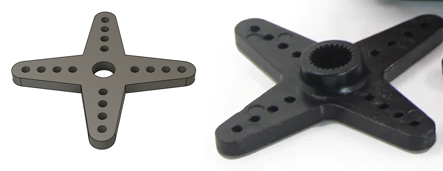
\includegraphics[scale=0.5]{quadthingmodelreal.png}
\caption{Modèle 3D et objet réel quadratique}
\end{figure}

\begin{figure}[H]
\centering
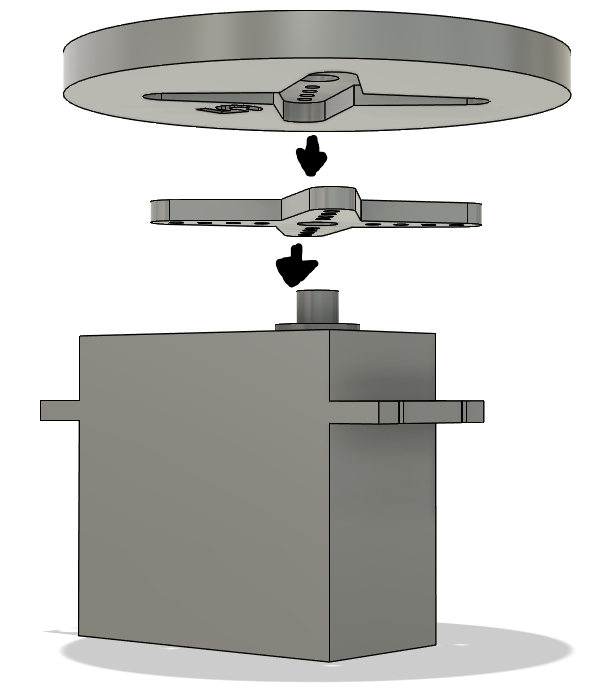
\includegraphics[scale=0.4]{wheelquadservo.png}
\caption{Emboitement des modèles}
\end{figure}

Une fois tout cela imprimé et monté il fallait tester l'adhésion des roues en 3D au cadenas. De base nous voulions tester avec un matériau en résine car il avait la même consistance que du caoutchouc, cela n'a pas été possible, nous l'avons donc imprimer en PLA. Cependant l'adhésion était nulle, la roue du cadenas ne tournait pas du tout. Le but étant de se rapprocher de l'adhésion de la roue par défaut, à savoir une matière en caoutchouc, l'idée de mettre des élastiques autour est donc apparue, et cela a fonctionné.
Pour faciliter la mise en place des élastiques sur la roue je l'ai modélisée à nouveau pour ajouter un U sur les bords (Voir Figure 6).

\begin{figure}[H]
\centering
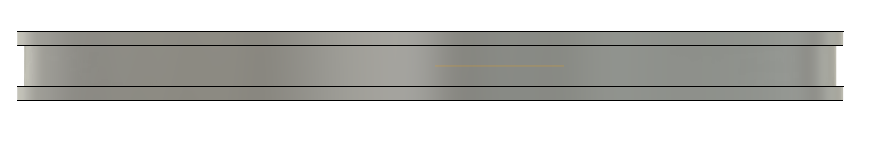
\includegraphics[scale=0.32]{wheelsU.png}
\caption{Rognage en U autour de la roue}
\end{figure}

Finalement un modèle 3D avec la caméra a du être réalisé, celle-ci devait être pile devant le cadenas à une distance de focus raisonnable d'environ 7cm. Ce premier modèle a donc été fait :

\begin{figure}[H]
\centering
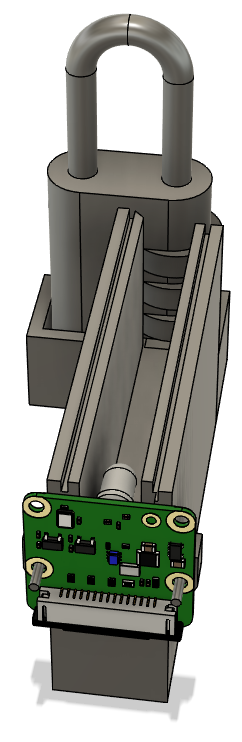
\includegraphics[scale=0.7]{cameralocker1ststruct.png}
\caption{1er modèle 3D pour la caméra}
\end{figure}

Ce modèle ne disposait que d'une seule LED, ce qui n'était pas suffisant pour que l'OCR détecte les chiffres, trois autres ont donc été ajoutées autour de la caméra. Une attention particulière au futur modèle a été apporté, la roue risquant de se coincer sur le modèle on a dû en couper le mur, ce pourquoi il est en diagonale.

\begin{figure}[H]
\centering
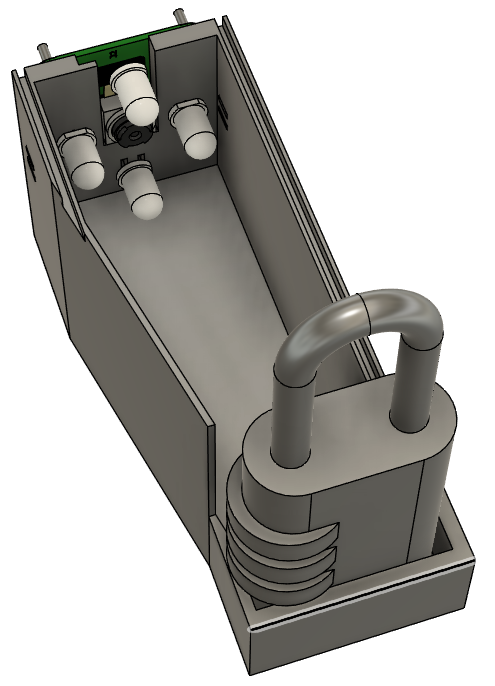
\includegraphics[scale=0.4]{cameralocker2dstruct.png}
\caption{2eme modèle 3D pour la caméra}
\end{figure}

Et finalement le modèle final, où l'on retrouve tout, c'est à dire, la caméra, le servo moteur avec sa roue, le cadenas, etc.

\begin{figure}[H]
\centering
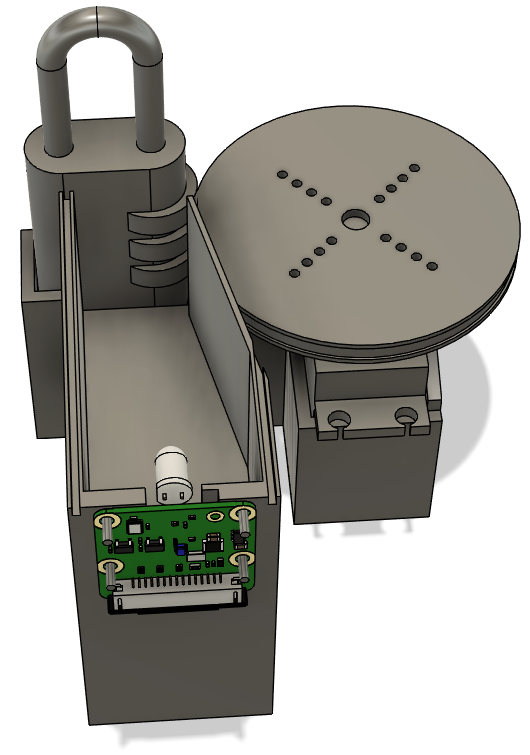
\includegraphics[scale=0.4]{lastModel.png}
\caption{Dernier modèle en 3D}
\end{figure}

Voici aussi ce modèle final en réel, avec le cadenas, le servomoteur et aussi le couvercle : 

\begin{figure}[H]
\centering
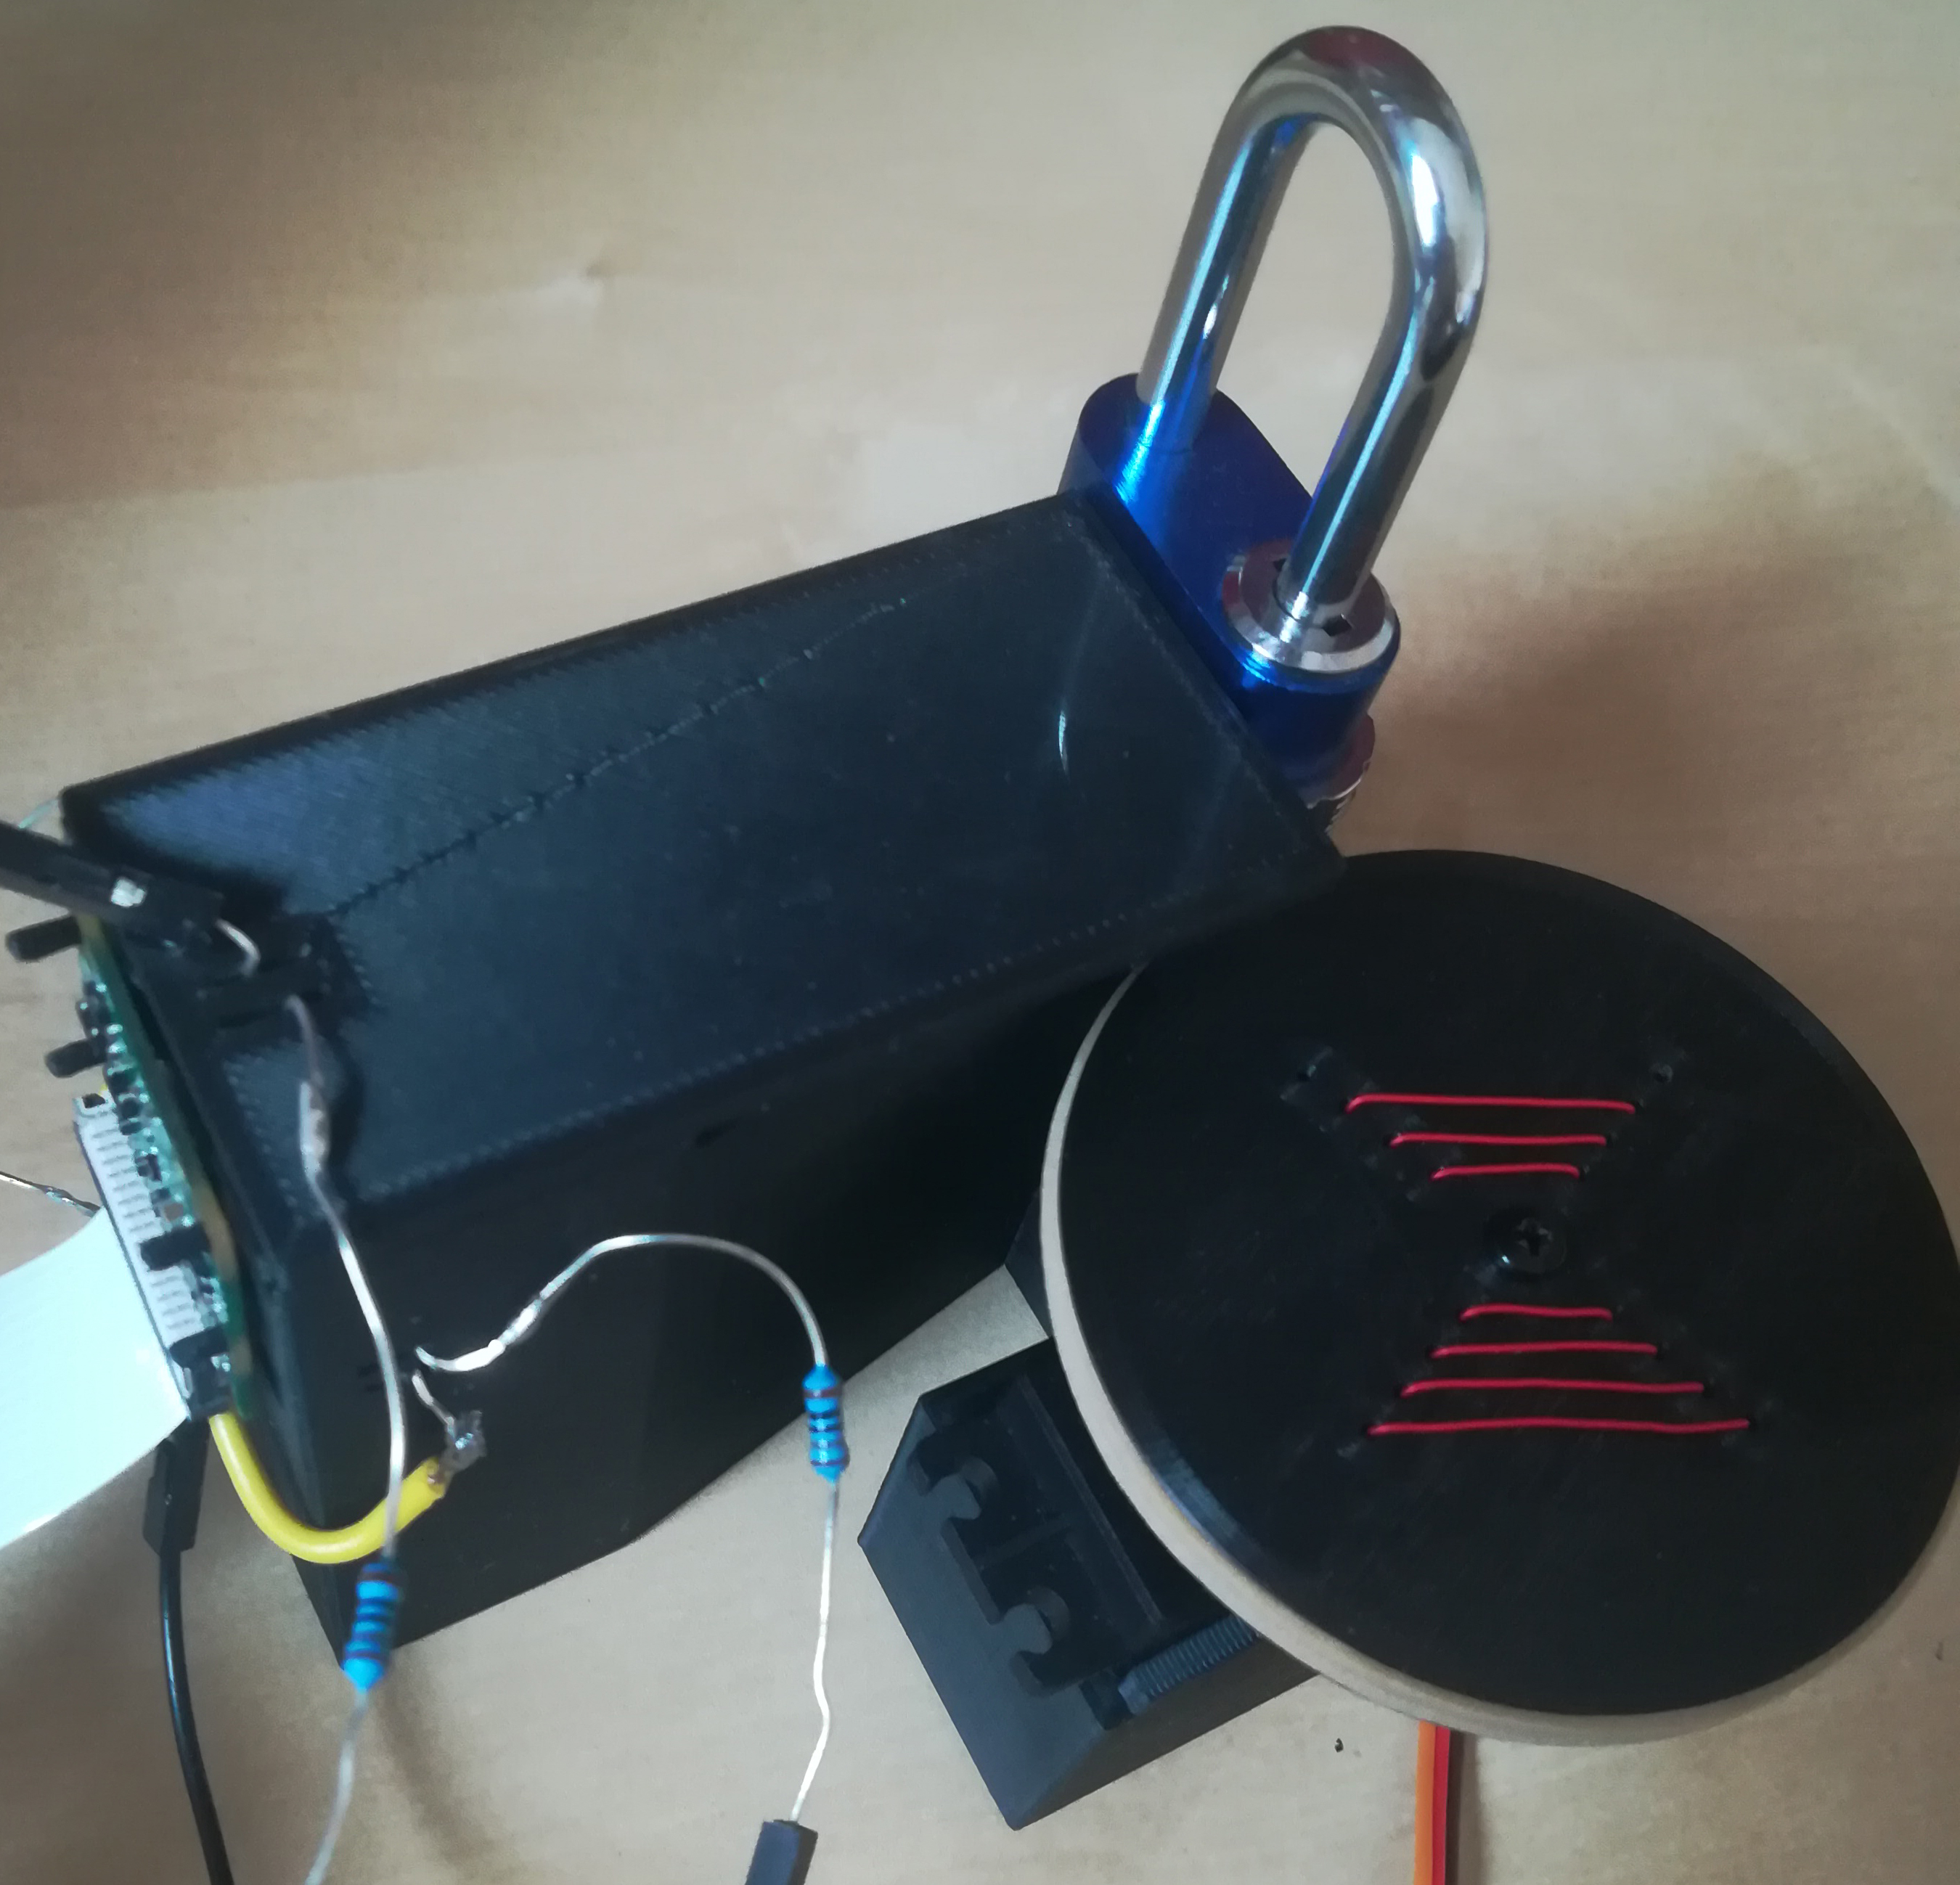
\includegraphics[scale=0.1]{modelefinalirl.jpg}
\caption{Dernier modèle en 3D}
\end{figure}

%------------------------------------------------

\section{Informatique}

De base je n'avais pas beaucoup de chose à faire pour l'informatique, si ce n'est coder le code pour contrôler le servomoteur. Comme tous les servomoteurs il est commandé par des impulsions et des délais, il y a peu de documentation à son sujet, je savais juste qu'il était commandable entre 500us et 2500us. Si l'on sait qu'un servomoteur à 3 états, à savoir une rotation dans le sens horaire, une autre dans le sens anti horaire et un état "stop". On peut supposer que ces 3 états ont une impulsion différente et séparé, j'en ai conclu qu'ils étaient à 1000us, 1500us et 2000us. Un autre document (Voir bibliographie) confirmait ma supposition. Un code simple a donc été fait pour contrôler le servomoteur sur arduino.

Par la suite, l'idée de rajouter une reconnaissance d'image a été amenée, l'arduino a été abandonné et la Raspberry Pi a pris sa place. Celle-ci pouvait aussi commander le servomoteur tout en ayant une caméra et avait accès à la reconnaissance d'image via tesseract-ocr.

Tout cela a été codé en python, l'idée est la suivante : Prendre une photo avec la caméra, faire du traitement d'image pour faciliter la lecture de l'OCR (Optical Character Recognition), l'OCR lit le chiffre après traitement, et finalement commande du servomoteur en fonction de la lecture.

La caméra est utilisée sur python via la librairie picamera, le traitement d'image se fait avec OpenCv, l'OCR utilise pytesseract (Un package qui permet d'utiliser tesseract-ocr sur python), pour le contrôle des Led (flash) et du servomoteur la libraire RPi.GPIO sera utilisée.

J'ai passé beaucoup de temps sur le traitement d'image, a essayé de la traiter pour que l'OCR puisse lire les chiffres plus facilement. En changeant le contraste, en faisant du treshold, en flouant l'image, en utilisant des systèmes propres à OpenCV comme de l'érosion (Éroder les pixels blancs sur l'image), parfois tout en même temps. Malheureusement rien de cela n'a été concluant. Voici un exemple de ce que je faisais lorsque je n'avais que une seule Led pour servir de flash : 

\begin{figure}[H]
\centering
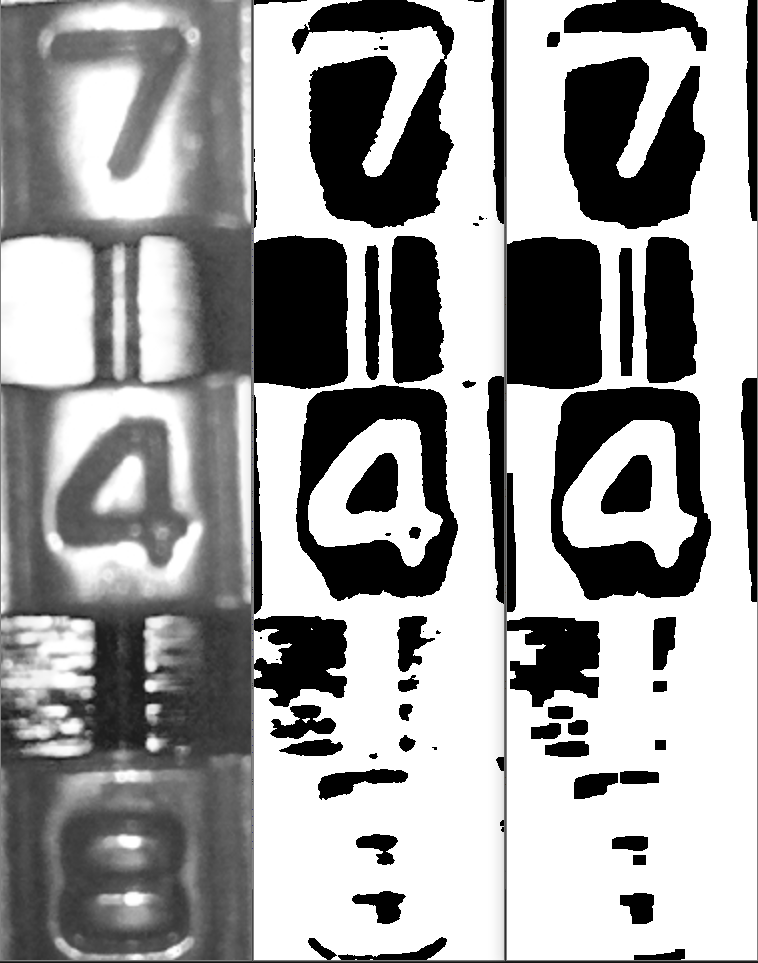
\includegraphics[scale=0.3]{TraitementImage.png}
\caption{Exemple traitement d'image}
\end{figure}

Premierement on remarque qu'un même traitement ne fonctionne pas pour les différentes rangées, le 8 devient illisible contrairement au 4 et au 7. Pour pallier ce problème j'ai rajouté plus de LED pour le flash. Cependant cela n'a pas réglé le problème général, à savoir que l'OCR ne sait pas reconnaitre le charactère parfaitement réalisé (Dans cette image-ci le 4).

Après discussion avec mes professeurs il est ressortit que le mieux serait d'entrainer l'IA (Intelligence Artificielle), contrôlant l'OCR, avec les images du cadenas. Pour que celle-ci puisse tout simplement mieux reconnaitre les caractères sans même devoir faire beaucoup de traitement d'image. Cependant, ceci dépasse le cadre de l'électronique et se rapproche plus de l'informatique. Et à ce moment là le temps étant proche de la fin de l'année scolaire, on trouvait qu'il était mieux que je finalise tout le reste, à savoir le modèle 3D final, et les codes pour tout contrôler.

\section{Améliorations possibles pour la suite}
Je vais expliquer ici les différentes améliorations possibles si le projet est repris une année suivante.

\subsection{Entrainement de l'IA pour l'OCR}

Comme expliqué dans la section informatique, le meilleure chose possible pour que l'OCR puisse détecter les chiffres est de l'entrainer. Cela est probablement la solution la plus efficace actuellement. Cependant il ne faudra pas négliger le traitement d'image qui devra quand même être un minimum présent.

\subsection{Servomoteur avec un couple plus faible}

Le servomoteur utilisé est le FS5103R, celui-ci à un couple de 3kg.cm/41.74oz.in. Il a suffisemment de couple pour pouvoir tourner les chiffres du cadenas, cependant il prends beaucoup de place. Ce que j'ai réalisé ne contient qu'un seul servomoteur, mais normalement il en faut trois. En essayant de faire un modèle avec trois servomoteur je me suis rendu compte que c'était extrêmenent compliqué car ils prennent beaucoup de place chacun. L'idée serait donc de vérifier si un servomoteur avec un couple plus faible, 1.5kg/cm par exemple, arrive à faire tourner les chiffres du cadenas. Parce que ceux-ci prendront moins de place et faciliterait donc la modélisation d'un modèle ayant trois servomoteurs.

\section{Conclusion}

En conclusion, la partie électronique est finie, la Raspberry Pi sert de cerveau pour le projet. Elle commande un servomoteur ainsi que des led et une caméra pour la reconnaissance d'image.

Plusieurs modèles 3D ont été réalisé pour convenir au mieux au besoin du projet et un boitier final a pu être réalisé dans les délais attendu. Une roue spécialisée a aussi été créer afin de pouvoir faire tourner le cadenas sans problème.

Finalement la reconnaissance d'image n'a pas été conluante , celle-ci n'est pas suffisante pour reconnaitre les caractères présent sur le cadenas malgré un tas de traitement d'image. Cependant la solution d'entrainer une IA afin d'arriver à la reconnaissance est prometteuse.
%----------------------------------------------------------------------------------------
%	REFERENCE LIST
%----------------------------------------------------------------------------------------

\begin{thebibliography}{99} % Bibliography - this is intentionally simple in this template

\bibitem{Datasheet}
Datasheet FS5103R, consulté en Février-Juin
\\{ \url{https://media.digikey.com/pdf/data\%20sheets/adafruit\%20pdfs/154_web.pdf}}
 
\end{thebibliography}

%----------------------------------------------------------------------------------------

\end{multicols}

\end{document}
